\chapter{Xây dựng UIT-OWL Editor}
\paragraph{Giới thiệu} Qua các chương trước, chúng em đã trình bày các cơ sở lý thuyết từ Semantic Web, Ontology Web Language và giới thiệu khái quát về OWL-API, Vaadin Framework- 2 công cụ chính xây dựng nên ứng dụng chỉnh sửa và phát triển Ontology trên Web mà chúng em tạm gọi là UIT-OWL Editor. Trong chương này, chúng em sẽ trình bày một cách chi tiết nhất có thể về quá trình xây dựng và phát triển nên ứng dụng này.
\section{Bố cục của ứng dụng}
\begin{figure}[h!]
	\centering
	\frame{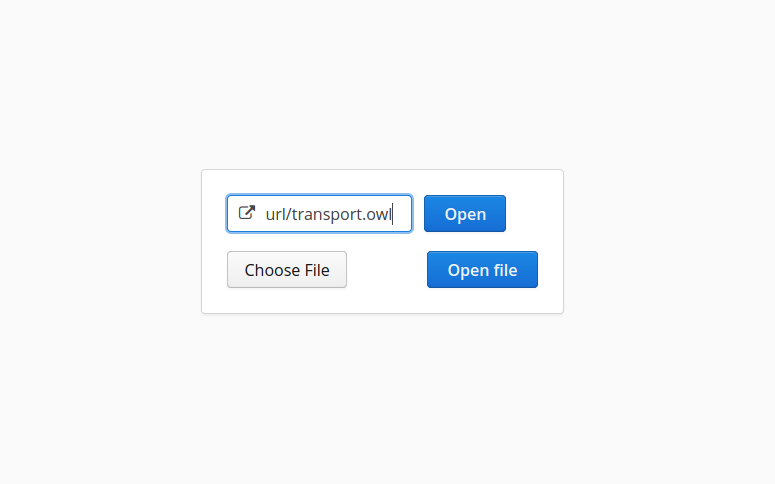
\includegraphics[width=100mm]{Figures/owleditor_entryview.png}}
	\caption{EntryView của UIT-OWL Editor\label{overflow}}
\end{figure}
\begin{figure}[h!]
	\centering
	\frame{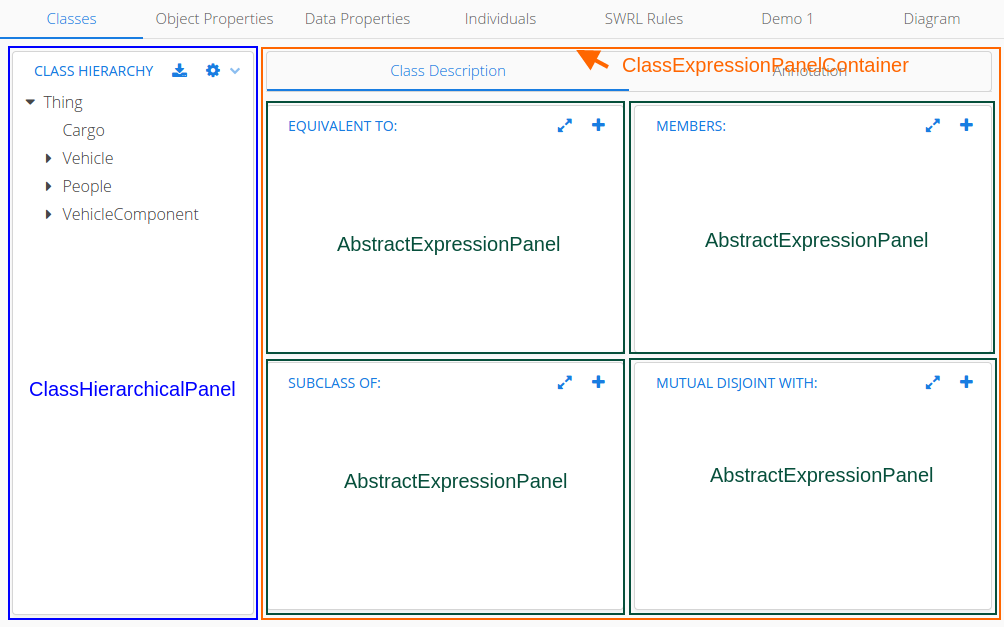
\includegraphics[width=150mm]{Figures/owleditor_mainview.png}}
	\caption{MainView của UIT-OWL Editor\label{overflow}}
\end{figure}
%
\subsection{Các view chính}
Ứng dụng UIT-OWLEditor chỉ gồm 2 View chính:
\begin{description}
\item[Entry View] tương đương với lớp \textit{vn.edu.uit.owleditor.EntryView} trong mã nguồn, là nơi chúng tập nhập vào URL của file OWL2 Ontology hoặc tải file OWL2 Ontology với các định dạng được trình bày trong chương 2.
\item[Main View] tương đướng với lớp \textit{vn.edu.uit.owleditor.MainView} trong mã nguồn,là giao diện chính của ứng dụng UIT-OWL Editor.
\end{description}
%
\subsection{Các tabsheet trong Main View}
Trong \textbf{MainView} sử dụng Component TabSheet các chứa các Tab tương ứng với các thực thể trong OWL2 Ontology, duy chỉ có 2 Tab cuối dùng để dùng làm demo tính năng phân loại là Tab Demo và Tab cuối cùng là Diagram dùng để vẽ các diagram, đồ thị về phân cấp các đối tượng trong OWL 2 Ontology.

% Class Tab
\subsubsection{Tab Classes} 
\begin{figure}[h!]
	\centering
	\frame{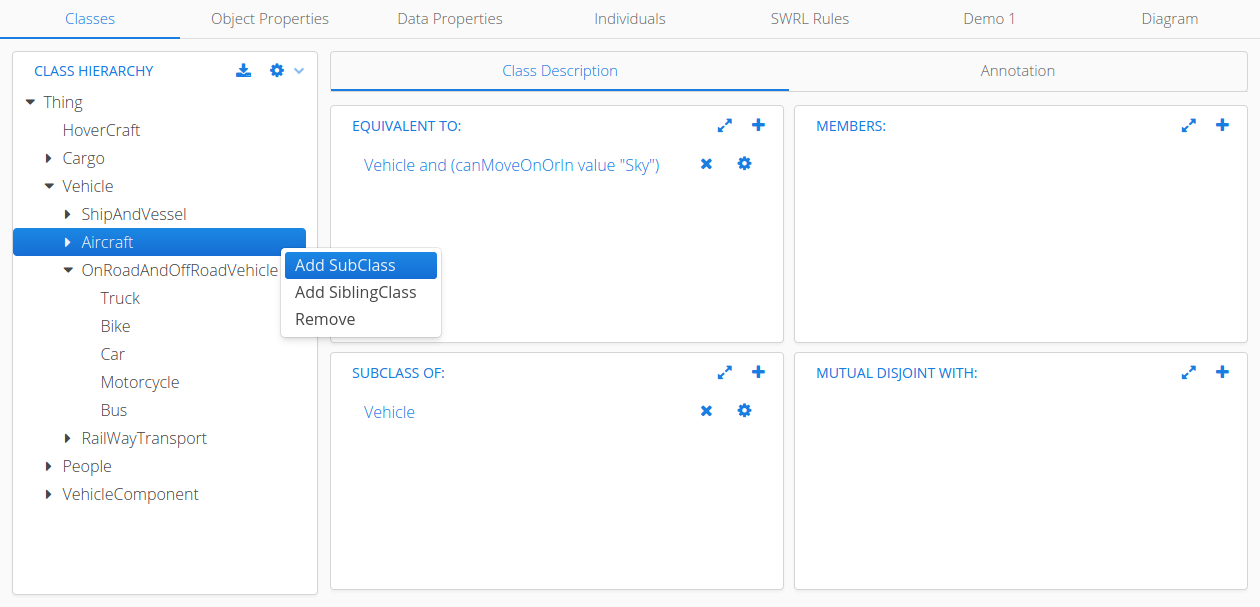
\includegraphics[width=150mm]{Figures/owleditor_classSheet.png}}
	\caption{Class Tab trong UIT-OWL Editor\label{overflow}}
\end{figure}
Tương ứng với lớp \verb|vn.edu.uit.owleditor.view.ClassesSheet| trong mã nguồn. Giao diện sử dụng HorizontalLayout của Vaadin gồm 
\begin{enumerate}
\item Panel bên trái là ClassHierachicalPanel có một cấu trúc dạng cây với các node chính là các lớp nằm trong OWL2 Ontology, với các chức năng thêm/xóa Sub/Sibling Class 
\item Các panel nhỏ bên phải được chứa trong lớp ClassExpressionPanelContainer, mỗ panel thể hiện một mô tả tương ứng với tên của panel đó.
\end{enumerate}	

% Object Property Tab
\subsubsection{Tab Object Properties}  
\begin{figure}[h!]
	\centering
	\frame{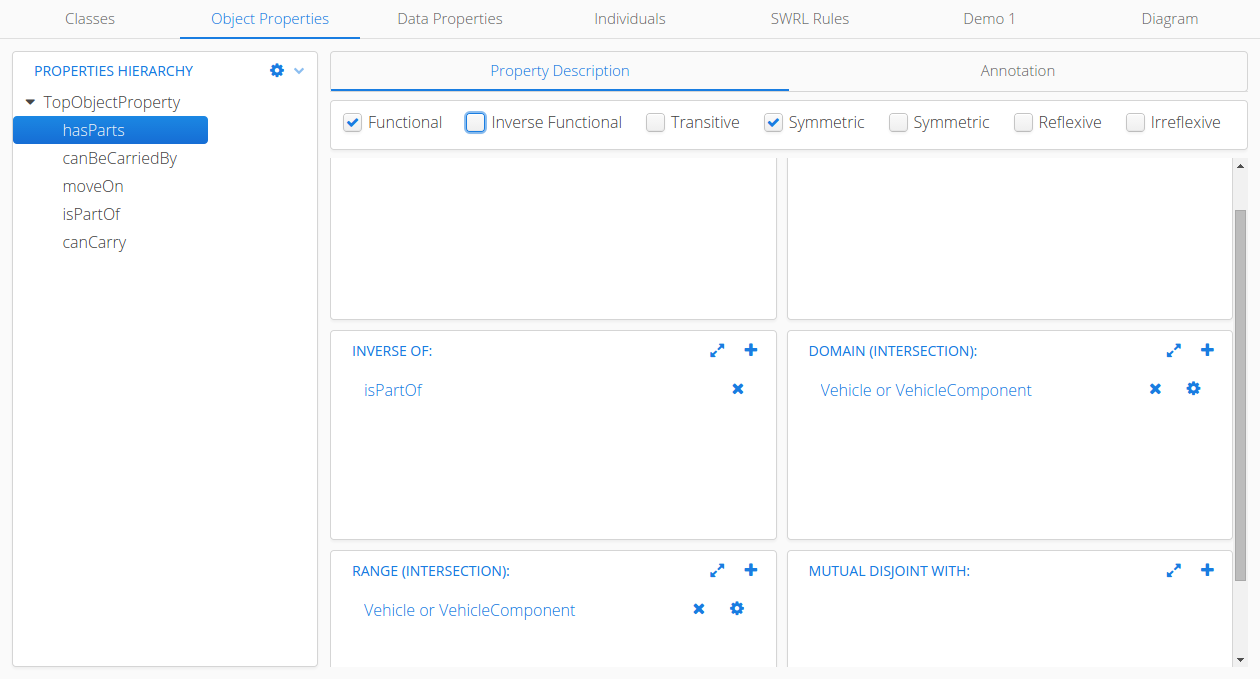
\includegraphics[width=150mm]{Figures/owleditor_opSheet.png}}
	\caption{Object Properties Tab trong UIT-OWL Editor\label{overflow}}
\end{figure}
Tương ứng với lớp \verb|vn.edu.uit.owleditor.view.ObjectPropertiesSheet| trong mã nguồn. Giao diện sử dụng HorizontalLayout của Vaadin gồm 
\begin{enumerate}
\item Panel bên trái là ObjectPropertyHierachicalPanel có một cấu trúc dạng cây với các node đại diện cho các thuộc tính đối tượng trong OWL2 Ontology, với các chức năng thêm/xóa Sibling/Sub Object Property.
\item Một dãy các \textit{CheckBox} dùng để thêm/xóa với các phát biểu trong mục 3.3.6.2 liên quan đến thuộc tính đối tượng được chọn bên trong cấu trúc cây ở bên phải.
\item Các panel nhỏ bên phải được chứa trong lớp ObjectPropertyExpressionPanelContainer, mỗ panel thể hiện một mô tả tương ứng với tên của panel đó về thuộc tính đối tượng đang được chọn trên cấu trúc cây.
\end{enumerate}	

% Data Property Tab
\subsubsection{Tab Data Properties}
\begin{figure}[h!]
	\centering
	\frame{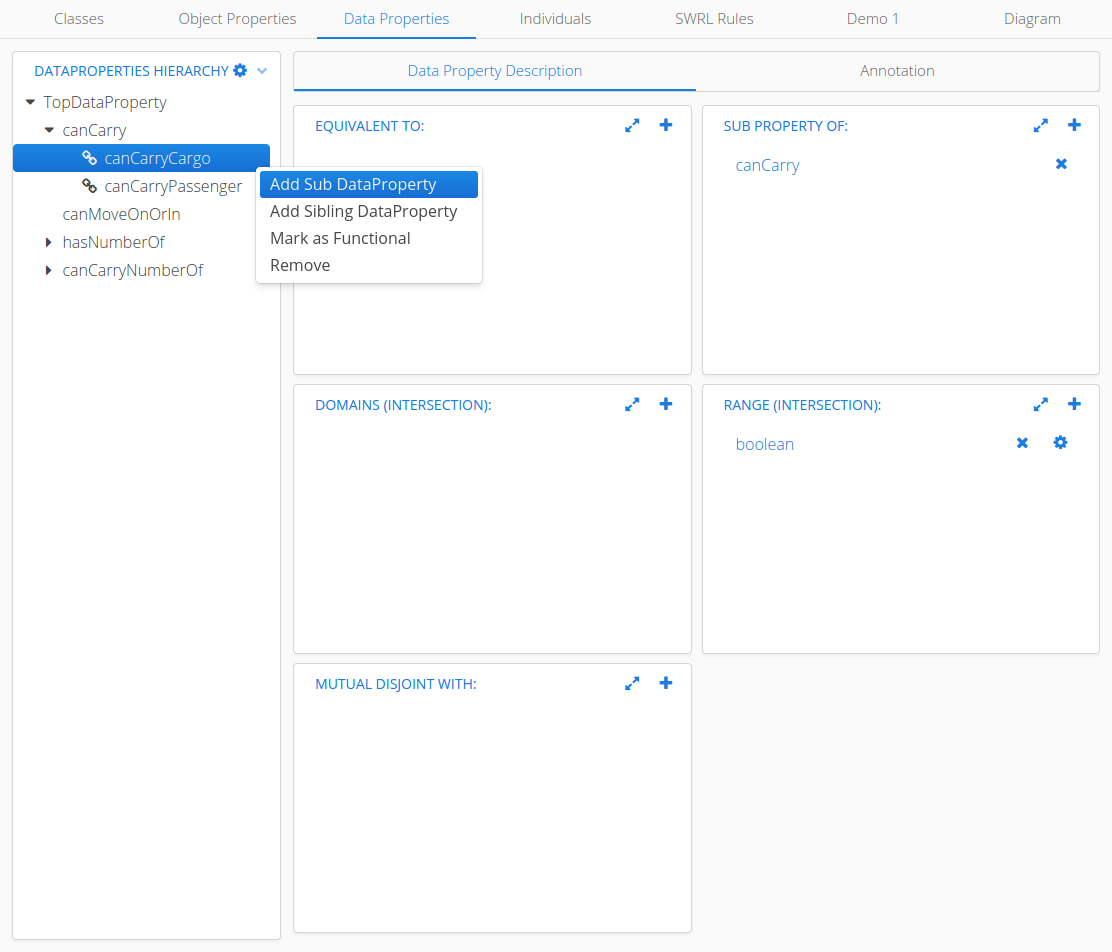
\includegraphics[width=150mm]{Figures/owleditor_dpSheet.png}}
	\caption{Data Properties Tab trong UIT-OWL Editor\label{overflow}}
\end{figure}
Tương ứng với lớp \verb|vn.edu.uit.owleditor.view.DataPropertiesSheet| trong mã nguồn. Các thành phần của tab này gồm:
\begin{enumerate}
\item Panel bên phải là DataPropertyHierachicalPanel có một cấu trúc dạng cây với các node đại diện cho các thuộc tính dữ liệu trong OWL2 Ontology, ngoài chức năng thêm/xóa Sibling/Sub DataProperty còn có tính năng thêm/xóa phát biểu FunctionalDataProperty (những thuộc tính nào có icon phía có nghĩa là có phát biểu FunctionalDataProperty về thuộc tính đó trong ontology.
\item Các panel nhỏ bên phải được chứa trong lớp ObjectPropertyExpressionPanelContainer, mỗ panel thể hiện một mô tả tương ứng với tên của panel đó về thuộc tính dữ liệu đang được chọn bên cấu trúc cây.
\end{enumerate}	

% Individual Tab
\subsubsection{Tab Individual}
\begin{figure}[h!]
	\centering
	\frame{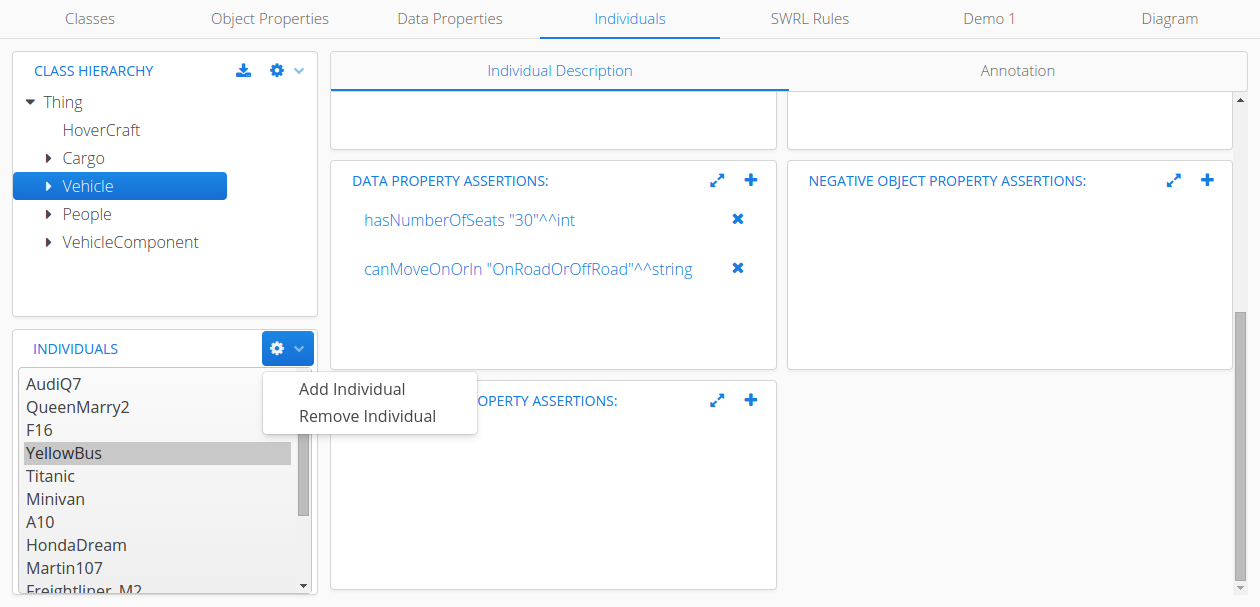
\includegraphics[width=150mm]{Figures/owleditor_individualSheet.png}}
	\caption{Individuals Tab trong UIT-OWL Editor\label{overflow}}
\end{figure}
Tương ứng với lớp \verb|vn.edu.uit.owleditor.view.IndividualsSheet| trong mã nguồn. Các thành phần của tab này gồm:
\begin{enumerate}
	\item Panel bên trái phía trên là ClassHierachicalPanel có một cấu trúc dạng cây với các node chính là các lớp nằm trong OWL2 Ontology, với các chức năng thêm/xóa Sub/Sibling Class. Khi chọn một lớp ở đây thì ListSelect ở bên dưới sẽ hiển thị một danh sách cá thể thuộc lớp này.
	\item Panel bên trái phía dưới là IndividualList hiển thị một danh sách gồm các cá thể thuộc lớp được chọn ở trên, có các tính năng thêm/xóa cá thể.
	\item Các panel bên phải là những panel biểu diễn các phát biểu assertion về cá thể. Tên panel cũng tương ứng với tên phát biểu trong OWL2.
\end{enumerate}

% SWRL Tab
\subsubsection{Tab SWRL}
\begin{figure}[h!]
	\centering
	\frame{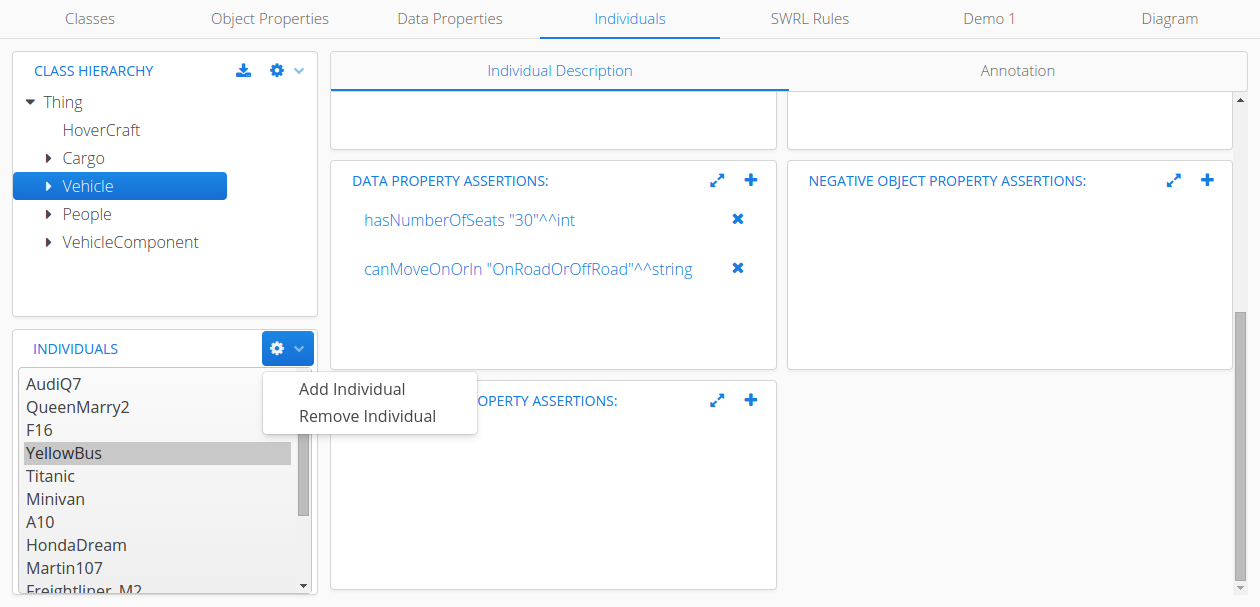
\includegraphics[width=150mm]{Figures/owleditor_individualSheet.png}}
	\caption{SWRL Rule Tab trong UIT-OWL Editor\label{overflow}}
\end{figure}
Tương ứng với lớp \verb|vn.edu.uit.owleditor.view.RuleSheet| trong mã nguồn. Tab này chỉ gồm một thành phần chính là một Table chứa các SWRL trong tài liệu OWL 2 Ontology. Khi right-click sẽ có các chức năng thêm/xóa/sửa rule được chọn.

% Demo Sheet
\subsubsection{Tab Demo}
\begin{figure}[h!]
	\centering
	\frame{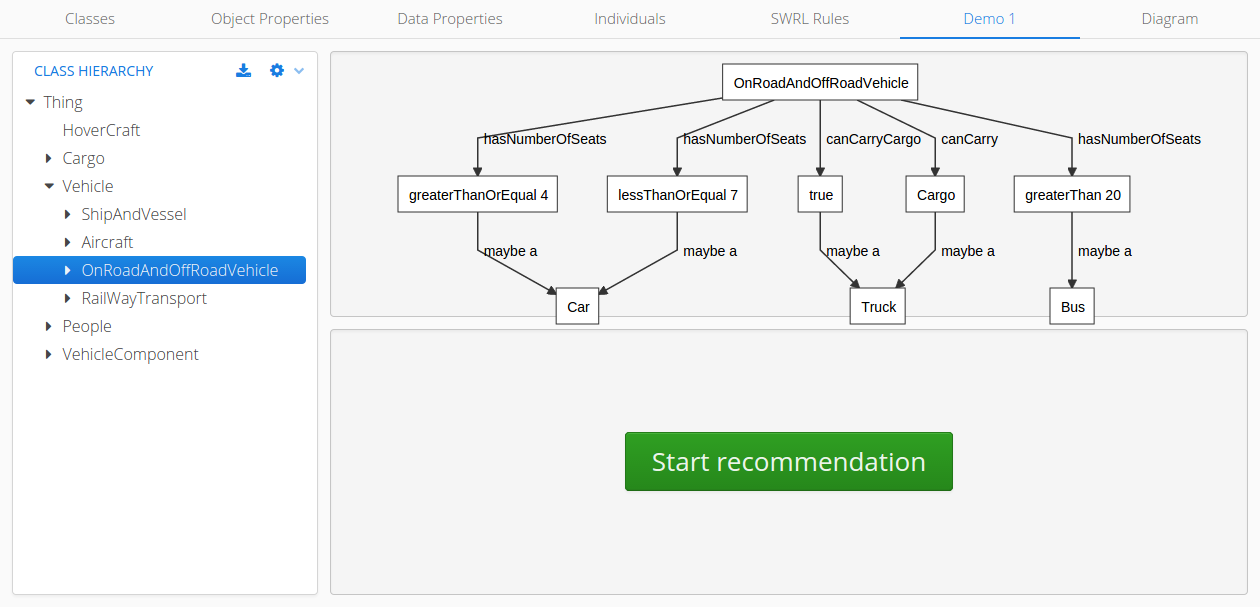
\includegraphics[width=150mm]{Figures/owleditor_demoSheet.png}}
	\caption{Demo Tab trong UIT-OWL Editor\label{overflow}}
\end{figure}
Demo Tab không nằm trong thành phần tiêu chuẩn mà một Ontology Editor bắt buộc phải có như các Tab đã giới thiệu. Tuy nhiên, chúng em cài đặt Demo Tab ở đây với mục đích thử nghiệm tính năng gợi ý phân loại dựa theo SWRL Rule, và sử dụng các Domain và Range restriction để hạn chế các giá trị mà người dùng có thể thêm cho vào cho một cá thể. Các thành phần của tab này gồm:
\begin{enumerate}
\item Panel bên trái là ClassHierachicalPanel.
\item Panel phía trên bên phải sẽ hiện thị một sơ đồ thể hiện gợi ý phân loại cho lớp được chọn.
\end{enumerate}}

%\section{Cấu trúc package của ứng dụng}
%\subsection{vn.edu.uit.owleditor}
%Chứa các đối tượng có vai trò là nơi đầu tiên code được thực thi khi người dùng gõ vào URL của ứng dụng. Gồm các đối tượng quan trọng sau
%\begin{description}
%\item[OWLEditorUI] là đối tượng được mở rộng (thừa kế) lớp \verb|UI| của Vaadin với chứng năng là nạp các component từ Entry 
%\end{description}
%\subsection{vn.edu.uit.owleditor.core}
%Gồm thành phần quan trọng nhất \verb|OWLEditorKit| (sẽ được trình ngay ở phần sau) và một số implementations của một vài interfaces trong OWL-API.
%\subsection{vn.edu.uit.owleditor.data}
%\begin{description}
%\item[vn.edu.uit.owleditor.data.hierarchy] Chứa các Data Model mở rộng từ lớp HierarchicalContainer của Vaadin.
%\item[vn.edu.uit.owleditor.list] Chứa các Data Model mở rộng từ lớp IndexedContainer của Vaadin.
%\item[vn.edu.uit.owleditor.property] Chức các Data Model implement interface Property của Vaadin.
%\end{description}
%\subsection{vn.edu.uit.owleditor.event}
%Chứa các sự kiện và các EventHandler Inteface của toàn ứng dụng UIT-OWL Editor.
%\subsection{vn.edu.uit.owleditor.view}
%Chứa các Tab vừa được nêu ở mục trên, EntryView và MainView.
%\subsubsection{vn.edu.uit.owleditor.view.component}
%Chứa các thành phần quan trọng như ClassExpressionEditor, AbstractExpressionPanel, SWRLRuleEditor.
%\subsubsection{vn.edu.uit.owleditor.view.panel}
%Chứa các Class/ObjectProperty/DataProperty HierarchicalPanel và ClassExpression/ObjectProperty/DataProperty/NamedIndividual PanelContainer
%\subsubsection{vn.edu.uit.owleditor.view.window}
%Chứa các lớp được mở rộng từ sub-window của Vaadin như build{Add/Edit}ClassExpressionWindow dùng để thêm/chỉnh sửa các mô tả lớp.
%\subsection{vn.edu.uit.owleditor.utils}
%Chứa enumeration OWLEditorData liệt kê các kiểu dữ liệu trong UIT-OWL Editor.
%\subsubsection{vn.edu.uit.owleditor.converter}
%Chứa các Converter tự định nghĩa được implement từ \textit{Converter} interface của Vaadin.
%\subsubsection{vn.edu.uit.owleditor.validator}
%Chứa các validator tự định nghĩa được implement từ \textit{Validator} interface của Vaadin.

\section{OWLEditorKit}
\begin{description}
\item[interface] vn.edu.uit.owleditor.OWLEditorKit
\item[class implementation] vn.edu.uit.owleditor.OWLEditorKitImpl
\end{description}
Đây là thành quan trọng nhất của toàn bộ ứng dụng đảm nhiệm việc khai thác các API từ OWL-API, nạp/tạo Ontology từ IRI, reasoning, giải thích các phát biểu, làm parser cho các mô tả lớp và dữ liệu. Thực ra, các chứng năng vừa kể trên hầu hết đều được thực thi nhờ các API củaj OWL-API, lớp này chỉ đơng giản đóng gói tất cả lại thành một đối tượng để dễ dàng sử dụng trong các UI Component hơn. Các chức năng của OWLEditorKit gồm:

\subsection{Load Ontology}
Tương ứng với hàm \textit{loadOntologyFromOntologyDocument}, load các tài liệu OWL2 từ đối tượng IRI của OWL-API, ontology khi load xong sẽ được gán cho đối tượng \verb|activeOntology|. 
\subsubsection{Active Ontology}
\begin{verbatim}
OWLOntology activeOntology;
\end{verbatim}
\verb|activeOntology| là một đối tượng được khai báo trong OWLEditorKitImpl. Mọi thay đổi về thêm/xóa/sửa các phát biểu qua các giao diện đều sẽ được cập nhật và áp dụng lên đối tượng này.
\subsubsection{OWLOntologyManager}
Là một dạng đối tượng tù thư viện OWL-API, đối tượng này được khởi tạo khi hàm OWLEditorKitImpl được khởi tạo.
\subsubsection{OWLDataFactory}
OWLEditorKit cũng có một OWLDataFactory đảm nhiệm việc xây dựng cá lớp/thuộc tính đối tượng/thuộc tính đối tượng dữ liệu, các mô tả lớp/thuộc tính và các phát biểu về lớp/thuộc tính cá thể.
\subsection{Reasoning}






















